%------------------------------------------------------------
\chapter{ 流体方程式の数値解法}
%------------------------------------------------------------

流体方程式は保存形式で表される。
\begin{equation}
    \frac{\partial {\bf U}}{\partial t} 
    + \frac{\partial {\bf F}}{\partial x}
    + \frac{\partial {\bf G}}{\partial y}
    + \frac{\partial {\bf H}}{\partial z}=0
\end{equation}
\begin{equation}
    {\bf U} = \left( 
        \begin{array}{c}
            \rho \\
            \rho v_x \\
            \rho v_y \\
            \rho v_z \\
            E
    \end{array}
\right),\;\;
    {\bf F} = \left( 
        \begin{array}{c}
            \rho v_x \\
            \rho v_x^2 + P \\
            \rho v_x v_y \\
            \rho v_x v_z \\
            (E + P)v_x
    \end{array}
\right),\;\;
    {\bf G} = \left( 
        \begin{array}{c}
            \rho v_y \\
            \rho v_y v_x \\
            \rho v_y^2 + P \\
            \rho v_y v_z \\
            (E + P)v_y
    \end{array}
\right),\;\;
    {\bf G} = \left( 
        \begin{array}{c}
            \rho v_z \\
            \rho v_z v_x \\
            \rho v_z v_y \\
            \rho v_z^2 + P  \\
            (E + P)v_z
    \end{array}
\right),\;\;
\end{equation}
%%%

\section{一次元数値流体計算コード}

\subsection{空間時間一次精度スキーム}

\begin{figure}[htpb]
    \centering
    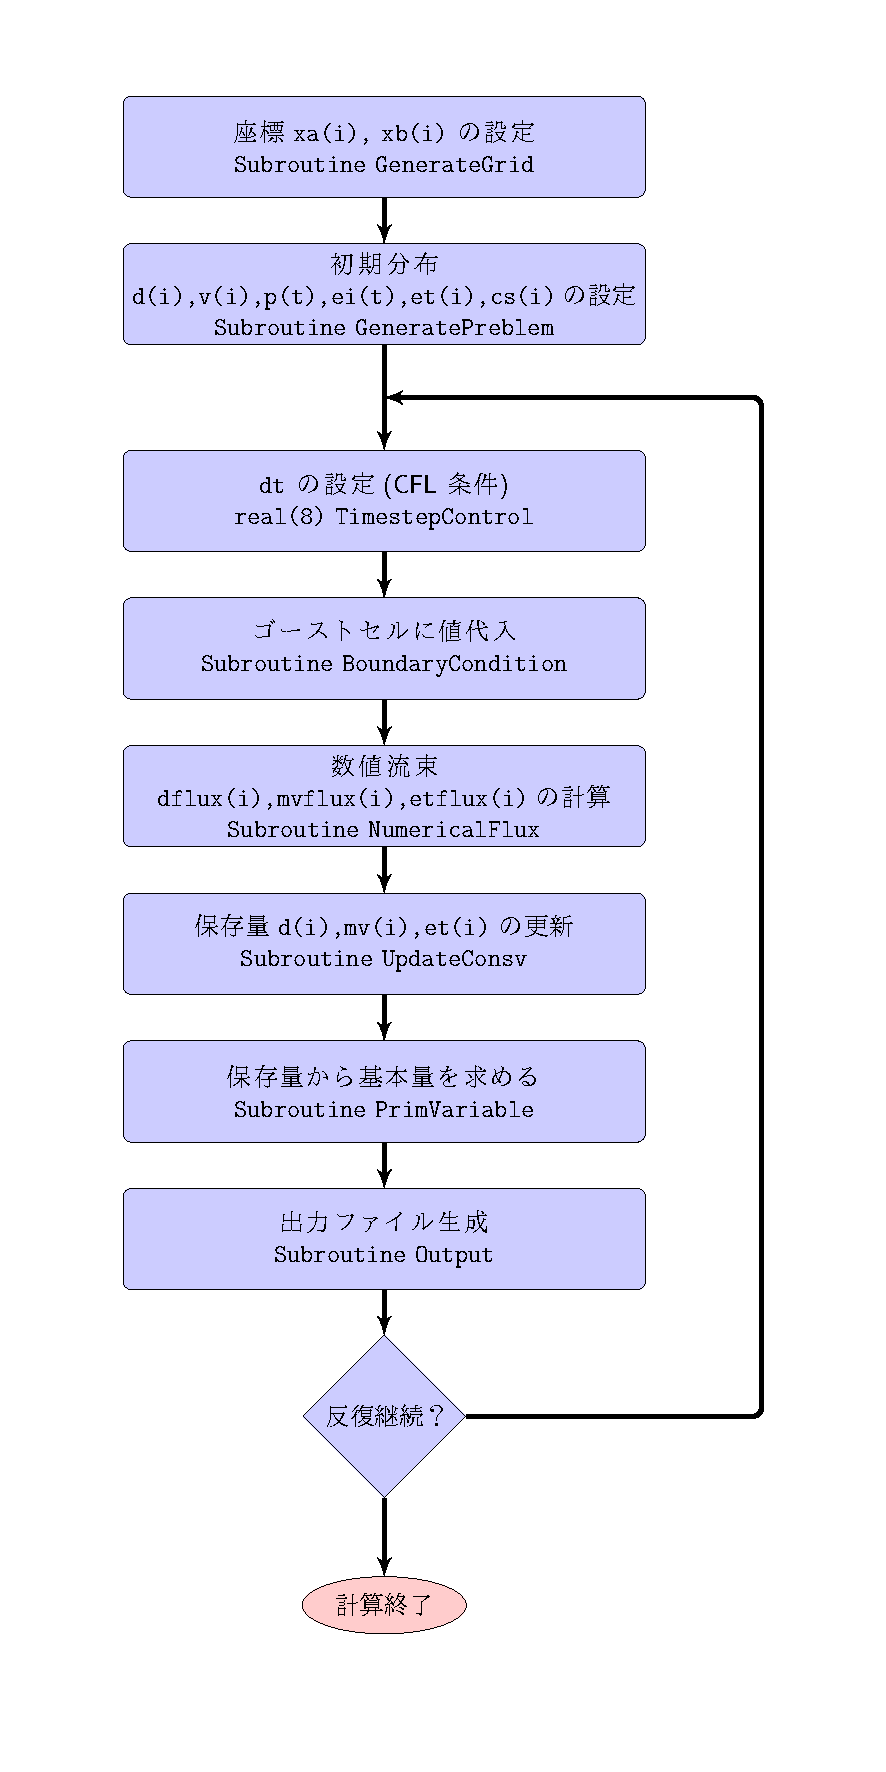
\includegraphics[width=8cm]{flowchart_HD1.pdf}
    \caption{サンプルプログラムの計算手順のフローチャート。
    }
    \label{fig:fc_FV2}
\end{figure}

\subsubsection{サンプルコードで使わている変数の説明}

\begin{table}[h]
\begin{center}
\caption{時間発展に関数する変数}
\begin{tabular}{|c|c|}
    \hline
    変数名/配列名 & 説明 \\
    \hline
    \hline
    {\ttfamily nhy} & 時間ステップ数 \\
    \hline
    {\ttfamily nhymax} & 最大時間ステップ数 \\
    \hline
    {\ttfamily time } & 時刻 \\
    \hline
    {\ttfamily timemax } & 計算終了時刻 \\
    \hline
    {\ttfamily dt} & 時間幅 \\
    \hline
\end{tabular}
\end{center}
\caption{ {\ttfamily nhy $>$ nhymax}または{\ttfamily time $>$ timemax}を満たすと計算が終了する。}
\end{table}

\begin{table}[h]
\begin{center}
\caption{座標に関する変数}
\begin{tabular}{|c|c|}
    \hline
    変数名/配列名 & 説明 \\
    \hline
    \hline
    {\ttfamily ngrid} & 計算領域内のセル総数 \\
    \hline
    {\ttfamily mgn} & ghost cell数 \\
    \hline
    {\ttfamily in} & ghost cellを含めたセル総数 \\
    \hline
    {\ttfamily is} & 計算領域左端のセル番号\\
    \hline
    {\ttfamily ie} & 計算領域右端のセル番号\\
    \hline
    {\ttfamily x1min} & 計算領域左端の座標 \\
    \hline
    {\ttfamily x1max} & 計算領域右端の座標 \\
    \hline
    {\ttfamily x1b(i)} & セル中心の座標 $x_{i}$ (要素数 {\ttfamily in-1}) \\
    \hline
    {\ttfamily x1a(i)} & セル境界の座標 $x_{i+1/2}$ (要素数 {\ttfamily in}) \\
    \hline
\end{tabular}
\end{center}
\end{table}


\begin{table}[h]
\begin{center}
\caption{流体変数に関する変数}
\begin{tabular}{|c|c|}
    \hline
    変数名/配列名 & 説明 \\
    \hline
    \hline
    \multicolumn{2}{|l|}{ {\bf 基本量} (primitive variables)} \\
    \hline
    {\ttfamily d(i)} & $x=x_i$における密度 (要素数 {\ttfamily in-1}) \\
    \hline
    {\ttfamily v(i)} & $x=x_i$における速度 (要素数 {\ttfamily in-1}) \\
    \hline
    {\ttfamily p(i)} & $x=x_i$における圧力 (要素数 {\ttfamily in-1}) \\
    \hline
    \multicolumn{2}{|l|}{ {\bf 保存量} (primitive variables) {\footnotesize 密度は基本量で出てくるので除いている}} \\
    \hline
    {\ttfamily mv(i)} & $x=x_i$における運動量 (要素数 {\ttfamily in-1}) \\
    \hline
    {\ttfamily et(i)} & $x=x_i$における全エネルギー (要素数 {\ttfamily in-1}) \\
    \hline
    \multicolumn{2}{|l|}{\bf その他の量} \\
    \hline
    {\ttfamily ei(i)} & $x=x_i$における内部エネルギー (要素数 {\ttfamily in-1}) \\
    \hline
    {\ttfamily cs(i)} & $x=x_i$における音速 (要素数 {\ttfamily in-1}) \\
    \hline
    \multicolumn{2}{|l|}{\bf セル境界の流束 (numerical flux)} \\
    \hline
    {\ttfamily dflux(i)} & $x=x_{i+1/2}$における質量流束 (要素数 {\ttfamily in}) \\
    \hline
    {\ttfamily mvflux(i)} & $x=x_{i+1/2}$における運動量流束 (要素数 {\ttfamily in}) \\
    \hline
    {\ttfamily etflux(i)} & $x=x_{i+1/2}$におけるエネルギー流束 (要素数 {\ttfamily in}) \\
    \hline
\end{tabular}
\end{center}
\end{table}




%一次元流体方程式を有限体積法を使って離散化すると,
%\begin{equation}
%    {\bf U}_{i}^{n+1} = {\bf U}_{i}^n 
%    - \frac{\Delta t}{\Delta x}\left( {\bf F}_{i+1/2}^{n+1/2} - {\bf F}_{i-1/2}^{n+1/2} \right)
%\end{equation}
%を得る。


